\documentclass[11pt]{article}
\usepackage{xcolor}
\usepackage{textcomp}
\usepackage{hyperref}
\usepackage{subcaption}
\usepackage{graphicx}
\usepackage{wrapfig}
\usepackage{amsmath}
\usepackage{array}
\usepackage[a4paper, margin=1in, footskip=0.25in]{geometry}

% relative path to images directory
% \graphicspath{ {./plots/} }
\newcommand{\round}[1]{\ensuremath{\lfloor#1\rceil}}
\setcounter{page}{0}


% make captions of figures cursive
\DeclareCaptionFormat{custom}
{
    \textbf{#1#2}\textit{\small #3}
}
\captionsetup{format=custom}
% \captionsetup{singlelinecheck=false}

\def\vdist{3ex}

\title{
	\textbf{Counteracting Erratic Behaviour:}\\
	\textbf{A Game-Theoretical Analysis of Parametrised Strategies}\\[6ex]
	\Large{High-School Thesis}\\
	\Large{(Maturaarbeit)}\\[\vdist]
	\Large{Mathematical-Computational}\\
	\Large{Analysis}\\[\vdist]
	\Large{Author:}\\
	\Large{Adrian Hossner}\\[3\vdist]
	\begin{flushleft}
		\begin{tabular}{>{\raggedright\arraybackslash}p{5cm} >{\raggedright\arraybackslash}p{5cm}}
			\Large{Supervisor: } & \Large{Geoffrey Ostrin}\\[\vdist]
			\Large{Submission Date: } & \Large{September 7, 2025}\\[\vdist]
			\Large{School: } & \Large{Gymnasium Thun}\\[\vdist]
		\end{tabular}
	\end{flushleft}
}
\date{ } % display no date

\begin{document}
\maketitle
\pagenumbering{gobble}

\newpage
\pagenumbering{arabic}

\section*{Abstract}
xxx

\newpage

\section*{Preface}
The present thesis has been written in times of global uncertainty.
At least partially, this is ascribed to a more or less erratic behaviour of political leaders, as a prime example the 47\textsuperscript{th} President of the U.S.A. Donald J. Trump.
When discussing this issue among my family and friends, a water-polo team member of mine drew my attention to the fact that this problem of erratic behaviour could be mathematically modelled by means of game theory.
Of particular interest in this context would be so-called Prisoner's Dilemma.
This game has been popularised in the 'A Beautiful Mind' film that narrates a story about the famous mathematician John Forbes Nash.
The resulting opportunity of combining my politically-social concerns with my subject-related interests in Computer Science and Mathematics captivated me immediately.
Hence, I was more than delighted that my school teacher Mr Ostrin accepted my request to serve as a supervisor of a related high-school thesis.\\
\indent Since then, Mr Ostrin has been always approachable and extremely valuable supporter of my work.
Likewise, I am grateful for all the help I have received from my parents, may it be as critical discussion partners, proofreader, or emotional coaches when I was stuck in problems. Many thanks from the bottom of my hearts!

\newpage

\tableofcontents
\newpage


\section{Introduction}
Interactions 

\begin{itemize}

	% Key idea:
	% Much uncertainty spread out because of (far-)right populists.
	% With insecurity comes random behaviour.
	% This simulations shows the difference of a random and a determined strategy.

	\item Interactions\\
		implication range is wide:\\
		from two persons in a relationship to countries in alliance\\
		from two impala's algrooming to zebras warning the herd about a lion \\
	% https://www.cell.com/trends/ecology-evolution/pdf/S0169-5347(00)88988-0.pdf

	\item Key hook:\\
		helping someone with possible cost -- cooperation\\
		being selfish but breaking trust -- defection\\

	\item Game Theory (optional, not needed for understanding)\\
		mathematical framework to investigate interactions\\

	\item model PD:\\
		single interaction\\
		already well analysed\\
		Nash found solution/equilibrium\\

	\item Iterated:\\
		more interesting, insightful\\
		strategies\\

	\item non-suited variants:\\
		Axelrod's Tournament\\
		Evolution\\

	\item continuous:\\
		more complex, accurate\\

	\item parameters:\\
		determines behaviour\\
		create surface\\
		the part that has not been experimented\\

	\item overall and difference:\\
		overall: wealth of population\\
		difference: competence between individuals\\

\end{itemize}

\section{Theoretical Foundations}

To grasp the game-theoretical approach pursued in this thesis, it is necessary to first understand the underlying key concepts. 
The most important ones being the Prisoner's Dilemma (PD) (2.1), the introduction of iterations as an extension (2.2) and the approach of submitting continuous values (2.3).
Furthermore, relevant information of published researches are provided as it seems helpful (2.5).

\subsection{Prisoner's Dilemma}
		
The Prisoner's Dilemma (PD) is a famous model in Game Theory. 
It was invented by Merrill Flood and Melvin Dresher in 1950. 
To understand the dilemma, a proper context has to be established.\\
Two persons are arrested and sued for having committed a crime jointly.
There is yet, however, insufficient evidence to imprison the two suspects.
Despite not having enough prove, the police utilises one of its methods.
They interrogate them separately without giving them a chance to coordinate beforehand.
The convicts receive two options.
On one hand, they can confess that the other suspect was involved in the crime. 
On the other hand, they have the right to remain silent.
Naturally, the police rewards the act of revealing the accomplice's delinquency over exercising the right of solidarity.
In case mutual trust and thus no confession took place, the twain separately receives an imprisonment of three years.
If both confess, either obtains five years in prison.
Nevertheless, by taking this course of action, this outcome is not the only existing.
If one chooses to confess while the other remains silent, the informer is released, whereas the betrayed must devote ten years in prison.
Remaining silent is considered as cooperation.
Whereby defection is the opposite, meaning breaking confidence and therefore state.
The following matrix visualises the pay-offs in this game in a comprehensive way:

% specific pay-off matrix
\begin{center}
\begin{tabular}{ c|c|c }
   & C & D \\ 
   \hline
 C & 3, 3 & 0, 10\\  
   \hline
 D & 10, 0 & 5, 5
\end{tabular}
\end{center}

\noindent
C represents cooperation and D corresponds to defection. 
The dilemma consists of the following.\\
The act of confessing appears alluring since there is a chance of eluding imprisonment.
Nonetheless, it is possible to receive five years in prison depending on the confederate's decision.
If the second criminal also confesses, both get five years in prison. 
This is the most inferior outcome for both which could have been avoided as either would have stayed silent.\\
John Nash, a mathematician which made great contributions in Game Theory, has proved the most reasonable course of action to be confessing.
The Nash-equilibrium is introduced. 
It defines a stable state in which both would not reconsider their own judgement although each of them would be aware of the other's decision.\\
This game composes a one-time interaction excellently in a mathematical and analytical perspective. 
The entitlement of the variables derives form the pay-off they suggest.\\
$T$: Temptation,
$R$: Reward,
$P$: Punishment,
$S$: Sucker's pay-off\\
The pay-offs in the matrix can be altered as long as these inequalities stay valid.
% \url{https://www.investopedia.com/terms/n/nash-equilibrium.asp}

% general pay-off matrix
\begin{center}
\begin{tabular}{ c|c|c }
   & C & D \\ 
   \hline
 C & R, R & S, T\\  
   \hline
 D & T, S & P, P
\end{tabular}
\end{center}

$$T > R > P > S$$

\subsection{Iterated}
		
The Iterated Prisoner's Dilemma (IPD) is a game which extends the PD. 
As the name suggests, the PD is played a number of times sequentially. 
To refer to the number of rounds played, $n$ is used as the denotation. 
The gained pay-offs accumulated over the last $n-i$ rounds are summed where $i$ represents the current round.
A strategy is an autonomous player which has its own behaviour.
Such a strategy has the whole history of the previous PDs at hand to generate the decision for the next round.
These decisions are calculated using conditions and probabilities that will be applied on the given data.
In this, and in the following variants, the analogy to the real world is changed.
Maximising one owns points is preferred.
Since a strategy strives to gain as many points as possible, the pay-off matrix must be altered accordingly.\\

\begin{center}
\begin{tabular}{ c|c|c }
   & C & D \\ 
   \hline
 C & 5, 5 & 10, 0\\  
   \hline
 D & 0, 10 & 3, 3
\end{tabular}
\end{center}

And to generalise this pay-off matrix as well, the numbers can be replaced with variables.
The concept is used for $T$, $R$, $P$, and $S$, provided that the four inequalities are satisfied.

\begin{center}
\begin{tabular}{ c|c|c }
   & C & D \\ 
   \hline
 C & R, R & S, T\\  
   \hline
 D & T, S & P, P
\end{tabular}
\end{center}

\begin{equation}
T < R < P < S\\
\end{equation}
\begin{equation}\label{eq:AvGrPa}
2R > T + S
\end{equation}

Inequality \eqref{eq:AvGrPa} is necessary to avoid receiving greater pay-offs by alternating cooperation and defection.\\
The Nash-equilibrium in the IPD differs from the that in the PD.
This implies that mutual cooperation yields long-term benefits.
Playing cooperation increases trust whereas defection allows exploitation.
Maximum pay-off during all the games is achieved only by consistent exploitation ($n \cdot T$).
Since persistent defection leads to mutual defection as a response, the practical attainment of the maximum points is severely limited.
To conclude, both strategies benefit the most with mutual cooperation.\\
A problem arises in the last round.
Since cooperation is only played to conserve trust, the reasonable action in the last round is to defect as trust has no use beyond the game.
If both strategies act rational, mutual defection will be played in the last round.
And because both are aware of this fact, there is no logical reason to cooperate the second last round.
This will end up in an inductive defection behaviour for both strategies the whole game.
So, to prevent constant mutual defection, the number of rounds played is an information that needs to be hidden from both strategies.
As a consequence of that, $n$ is a random number whose limits can be defined.\\
This extension of the PD allows to simulate a relationship of two individuals.

\subsection{Continuous}

In this variant, strategies are not limited to either cooperate or defect; instead, they can chose any level of cooperation between 0 and 1.
It is thus named Iterated Continuous Prisoner's Dilemma (ICPD)
This cooperation level, called investment or contribution, ranges from zero (defect) to one (cooperate).
The continuous form offers enhanced precision and mathematical applicability.\\
% One would suspect a very similar pay-off system to the iterated variant.
% In the discrete version, it looked like this:
%
% \begin{center}
% \begin{tabular}{ c c }
% Pay-off Player A & Pay-off Player B\\
% \begin{tabular}{ c|c|c }
%    & $C_A$ & $D_A$ \\ 
%    \hline
%  $C_B$ & 3 & 5\\  
%    \hline
%  $D_B$ & 0 & 1
% \end{tabular}
% &
% \begin{tabular}{ c|c|c }
%    & $C_A$ & $D_A$ \\ 
%    \hline
%  $C_B$ & 3 & 0\\  
%    \hline
%  $D_B$ & 5 & 1
% \end{tabular}
% \end{tabular}
% \end{center}

Two main approaches will be presented and evaluated for practicality in this thesis.
First, an intuitive extension of the iterated form. And second, a way that simplifies mathematically analysability.\\
A similar concept can be used to calculate the pay-offs given the investments of both strategies.
This concept is referring to a matrix-like pay-off system.
To include continuous values, a mathematical procedure is applied to the discrete version of the matrix, namely bilinear interpolation.
This will establish a field that can be represented by colour grades, a heat map.
Please see Figure \ref{fig:heatmaps}.
The equation used to calculate this heat map can be found in the Appendix.

\begin{figure}[h]
	\centering
	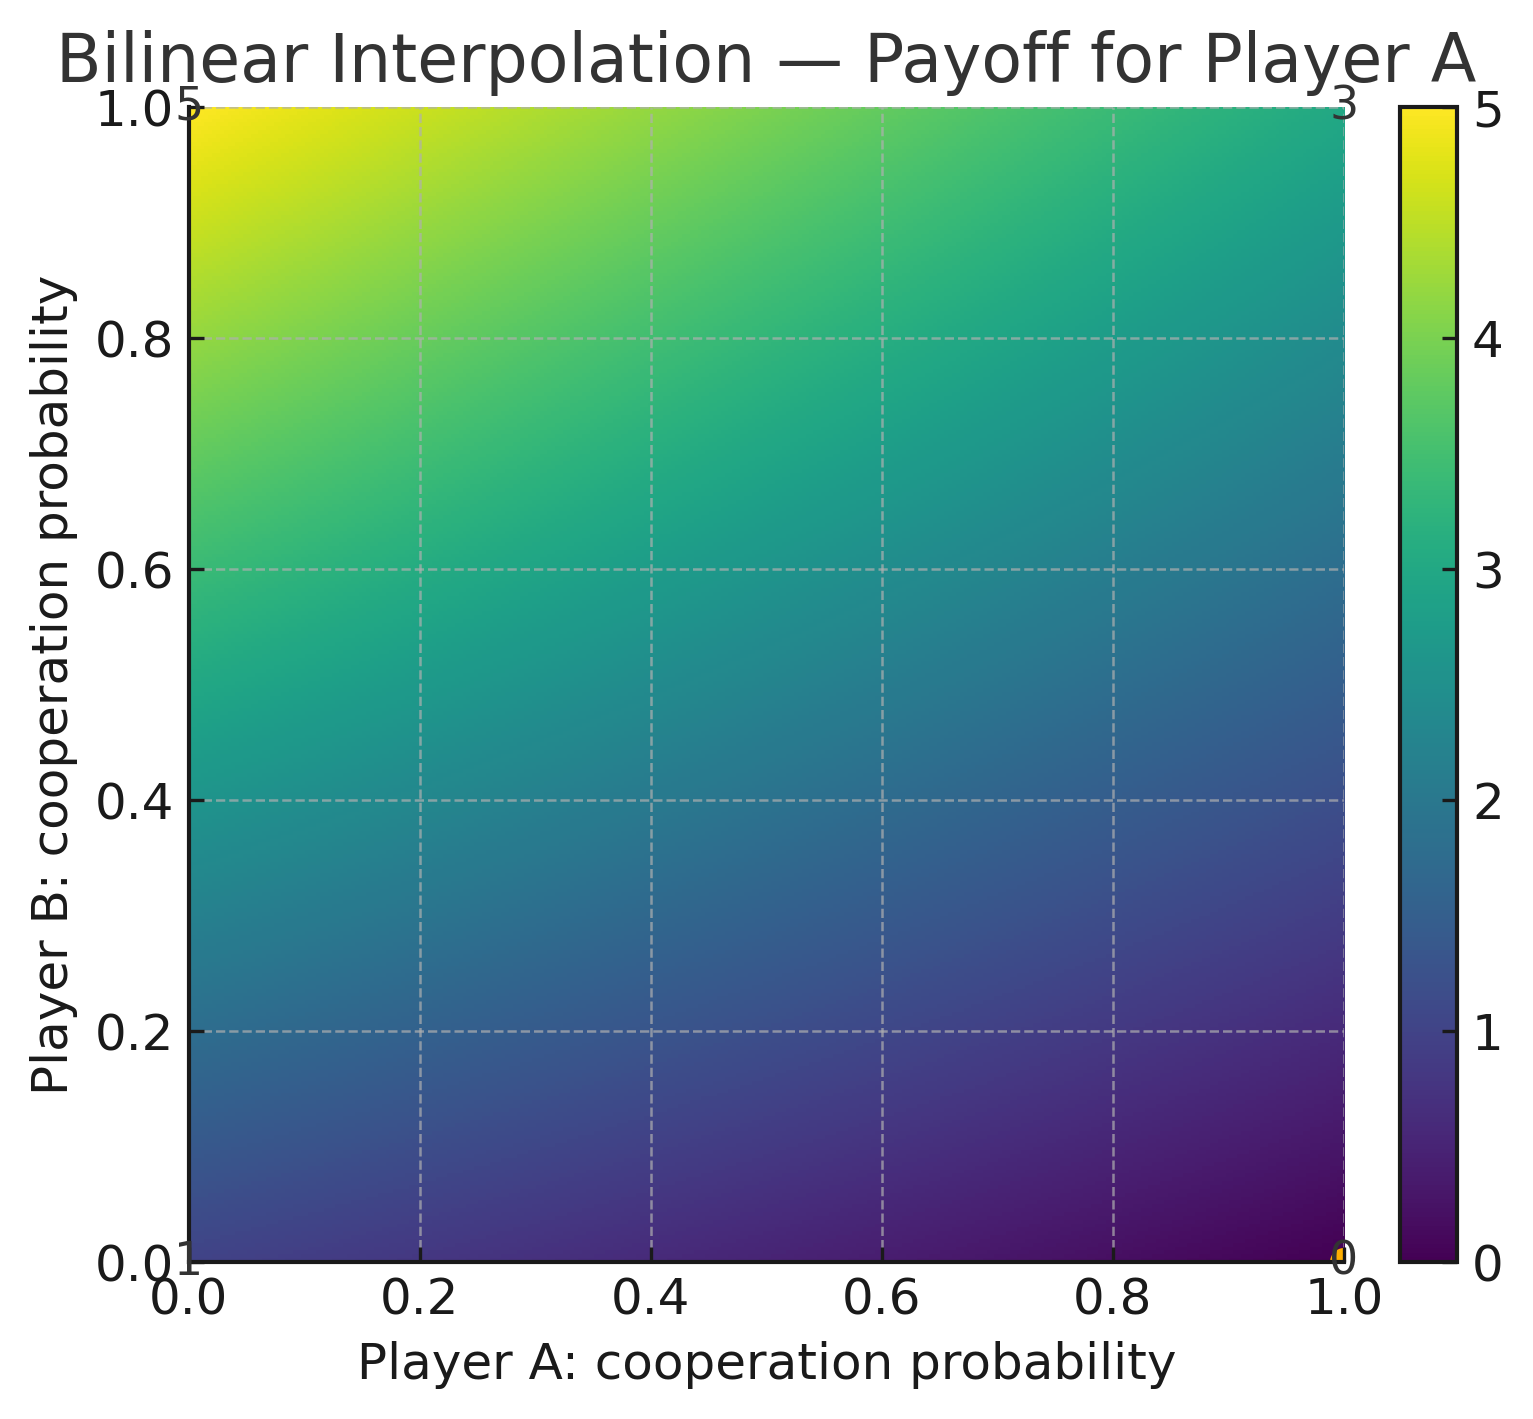
\includegraphics[width=0.45\textwidth]{images/pd_heatmap_A}\hfill
	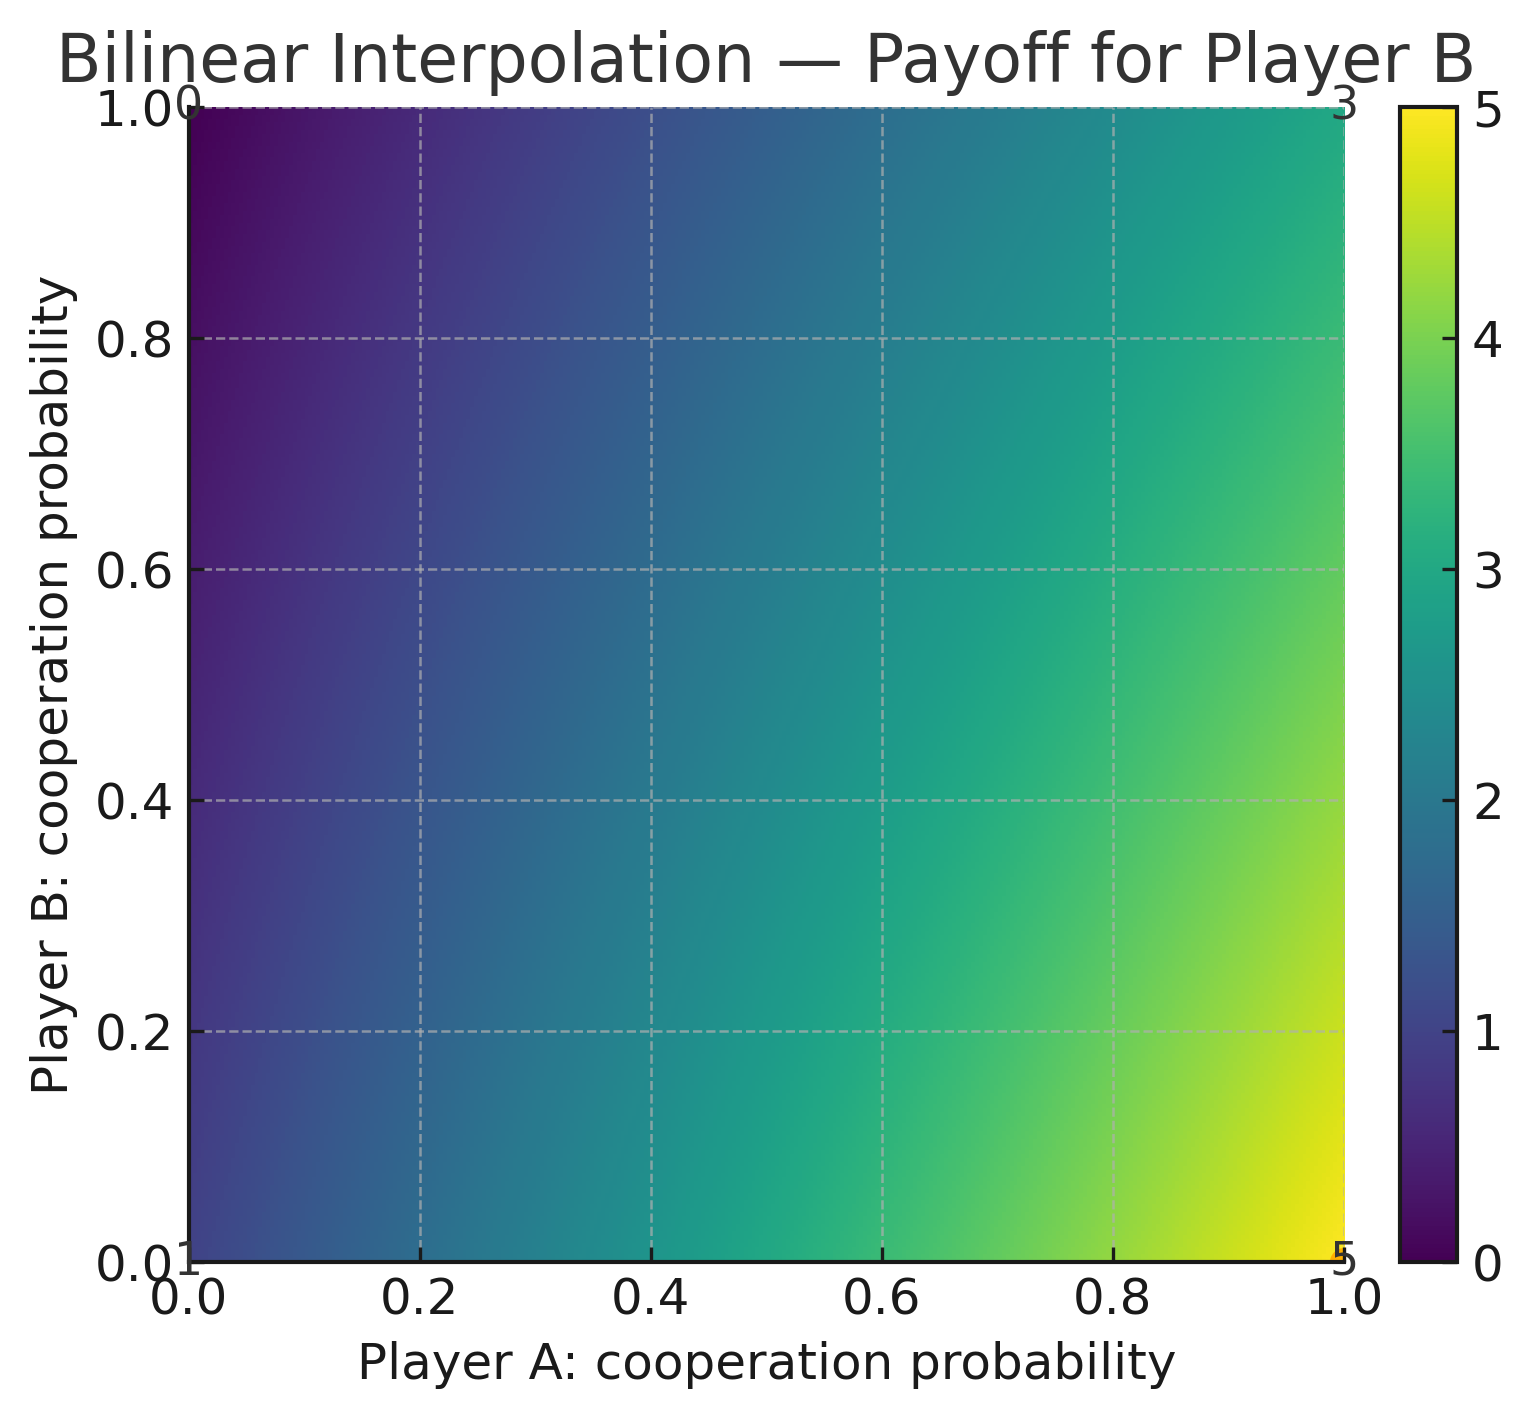
\includegraphics[width=0.45\textwidth]{images/pd_heatmap_B}
	\caption{Pay-off heat maps in the ICPD.}
	\label{fig:heatmaps}
\end{figure}

% I used ChatGPT-o4 to generate these heat maps.
% It generated them using these functions:
%
% $$U_A = (1-x)(1-y)R_A + (1-x)yS_A + x(1-y)T_A + xyP_A$$
% $$U_B = (1-x)(1-y)R_B + (1-x)yS_B + x(1-y)T_B + xyP_B$$
%
% These functions are applied to every point on the map.
% The variable x is the investment of strategy A and y is the investment of strategy B.
The second approach utilises only equations instead.
This pay-off system of [sciencedirect.com] is formed by:

$$p_A = y - c \cdot x + c$$
$$p_B = x - c \cdot y + c$$

$p_A$ and $p_B$ are the pay-offs of strategy A and B respectively.
$x$ is the investment of strategy A and $y$ is that of strategy B.
The coefficient $c$ ranges, as well as x and y, from 0 to 1 and describes the cost-to-benefit ratio.
The pay-off is highly influenced by the opponent's investment.
Only a fraction of one owns contribution is subtracted, $c$ being the coefficient.
The minimum pay-off one strategy can collect is then $-c$.
To avoid negative pay-offs and enhance subsequent convenience, a third addend is appended, $c$.
So, the least points that can be gained is 0.
The maximal points, which can be earned by exploitation, is $1 + c$.


% Let's see if the principles of the initial PD are still valid.
% It is better for one to defect (submit a 0) to get rid of the subtraction.
% And it is better for the strategy if the opponent's cooperates.
% If both defect, one gets zero points.
% If both cooperate, both get one point.
% If, however, one strategy exploits the opponent, meaning it defects while the other cooperates, it will get the maximum points being 1.
% The opponent would then get $-c$ points.
% This is the least one can receive.

		% 0 to 1 rather than cooperation or defection\\
		% Pay-off system\\ % https://www.sciencedirect.com/science/article/pii/S0022519306004255?casa_token=hIA0lYvzjf8AAAAA:Up2uQ89wotaLz7s1R0dM2FK7SaulAo40wIM-BdM9yooZ8uJeRL6mPs-K55dPNGs4XkcclNVjDQ#aep-section-id24
		% more accurate\\
		% more complex, generates more data \textrightarrow more insightful\\

\subsection{Additional variants}

There exist several extensions of the PD that will remain untouched in this thesis, one of which is noise, meaning that investments are altered with a certain probability.
This noise is introduced to simulate misunderstandings.\\
Another advancement being the alternating form.
In this variant, investments are contributed in succession rather than concurrently as in the conventional simultaneous model.\\
The evolutionary research domain surveys the success of strategies in a world where natural selection takes place.
This implies that losing strategies vanish, while successful ones replicate.

% \subsection{Noise}
%
% Noise in the ICPD is the equivalent to miscommunication or misunderstanding in the real world.
% In this variant of the PD, noise is essential to trigger interesting outcomes.
% When a game of the ICPD is started and two strategies who start with a full investment, many strategies only respond with full investments.
% So noise is necessary to trigger continuous investments. 
% Without noise, in many cases, the ICPD would be equivalent to the IPD.
%
% 		% sometimes necessary to trigger continuous investments\\
% 		% simulates misunderstandings\\
%
% \subsection{Simultaneous vs Alternating}
%
% Two main differences can be seen when simulating an iterated variant of the PD.
% On one hand there is the simultaneous form whereby the strategies submit their contribution at the same time.
% On the other hand, there is the alternating form in which on e strategy submits its contribution and the other strategy can respond to this contribution is that round.
% Since the alternating form gives and advantage to the strategy which is allowed to respond, this only makes things more complicated than necessary.
% So, this analysis is only dedicated to the simultaneous form.

\subsection{Current Findings}

Axelrod's Tournament
In the simpler variants, e.g. the IPD without noise, it has been proved many times over that the strategy Tit-For-Tat is the most successful one. [sources]
The success of strategies, however, can vary depending on certain conditions such as the influence of noise or different pay-off systems where continuous investments can be submitted.
So, the very specific area of the simultaneous ICPD, has not been very well explored.
...

\section{Methods and Implementation}

For answering the central research question, it was necessary to develop a overarching study design (3.1), to specify the strategies that will be pursued in the iterated continuous Prisoner’s dilemma (3.2), and to determine details of the implementation in terms of IT (3.3).

\subsection{Study design}

Erratic behaviour in respect of the PD can be equated to a random conduct.
Three strategy-types are proposed by reason that counter such erraticism.
Hereunto can a strategy either be unaffected and behold its manner of responding or react to the randomness.
In the former case, strategies are identified as rigid.
Whereas the latter is characterised as adaptive.\\

All of these categories of behaviour can algorithmised differently.
This particularly concerns the above introduced distinction of the discrete and the continuous form.
Applied to the erratic strategies, this means that the investment is a substantial random number between zero and one.
In contrast, the discrete version of this strategy generates a random number that is then rounded to the nearest integer.
The same approach hold true in the adaptive strategy.
Discrete contributions of rigid strategies are equal to either always cooperating (AlwaysCooperate) or constantly defecting (AlwaysDefect).
Whereas continuous strategies of the rigid category contribute continuous investments invariably, e.g. 0.5 (AlwaysNeutral).\\

Furthermore, it is possible to specify the extremeness of each behaviour.
This means that the randomness of an erratic strategy, the adaptiveness of an adaptive strategy and the investment of a rigid strategy can be defined.
On this account, a parameter is incorporated into the determination of the investment and the evaluation of various conditions.
It has, incidently, never been undertaken in this manner in the history of researches that concern the ICPD.\\

To keep the number of comparisons manageable within the realms of a Maturaarbeit (MA), five strategy were chosen.
Firstly, the selected strategies in the random class were named to be a discrete (Random-Discrete) and a continuous (Random-Continuous) version.
Secondly, the same concept was established in the adaptive category with the discrete (Adapt-Discrete) and the continuous (Adapt-Continuous) behaviour.
These strategies hold a parameter which determines the peculiarity level and ranges from zero to ten.
So ultimately, the discrete and the continuous implementation are included in one strategy (AlwaysSame) due to this parameter.
Thus, the distinction of a discrete and a continuous design would be trivial.\\


% Surfaces:\\
%
% The end result of this paper will be several surface plots.
% The data will be generated by letting two parameter-based strategies play against each other the ICPD.
% The game will be structured so that every parameter came against every other parameter in the ICPD.
% In total, I will let them play the ICPD 100 times in order to smooth out abnormalities which happen only once.
% Like this, a surface can be plotted by having the x-axis being the parameter of strategy 1 and the y-axis being the parameter of strategy 2.
% The z-axis will indicate the points one strategy gained.
% Since there are two strategies in one game, one surface will be shown for each strategy.
% Further more, the two z-axis of the two surfaces can be added and form a new surface which shows the overall points gained by both strategies.
% The complement to that would be to subtract the two z-axis to plot a surface showing the difference between the two surfaces.
% This describes how much better one strategy was than the other.
% So, in the end there will be four surface plots per one ICPD.
%
		% Let two strategies play ICPD\\
		% let every parameter play against every other parameter\\
		% parameters as x and y-axis, points as z-axis\\
		% one surface for each strategy\\
		% overall surface is population wealth (addition)\\
		% difference surface is individual competence (subtraction)

\subsection{Implemented Strategies}

As justified before, five strategies, namely Random-Discrete, Random-Continuous, Adapt-Discrete, Adapt-Continuous and AlwaysSame, will be presented and specified in the following.
	
\subsubsection*{Adapt-Continuous}
Adapt-Continuous (AdpC) is an, as the name suggests, adaptive and thus responsive strategy.
It starts with full cooperation to offer a constructive relationship within this simulation.
After having played one round, it will adapt to the submissions of the opponent by shifting its own investment towards the opponent's.
$$i_k(\theta_{\mathrm{AdpC}}) = i_{k-1} + s(\theta_{\mathrm{AdpC}}, k)$$
$$s(\theta_{\mathrm{AdpC}}, k) = \frac{\theta_{\mathrm{AdpC}}}{5} \cdot (\bar i_{k-1} - i_{k-1})$$
$k$ indicates the current round and is used to notate the equations recursively.
$k$ only appears in the adaptive strategies as only they require information of the past rounds.
The shift being applied to its own previous investment is notated with the function $s(\theta_{\mathrm{AdpC}})$.
This strategy with the parameter 0 is identical to AlwaysCooperate since the difference and thus the shift is multiplied by 0.
Dividing $\theta_{\mathrm{AdpC}}$ by 5 implies the fact that this coefficient to the difference is equal to one if the parameter equals five.
This means that the strategy will shift its next investment to exactly the previous investment of the opponent.
This behaviour corresponds to Tit-For-Tat.
$\theta_{\mathrm{AdpC}} = 10$ also shows an interesting nature of the strategy.
By having the parameter set to ten, it means Adapt will add the shift to its own previous investment twice.
Of course, one strategy is not allowed to submit any investment that exceeds the limits that is defined to be from 0 to 1.
The implementation of this strategy will simply set its investment to the reached limit if surpassed.\\

\subsubsection*{Adapt-Discrete}
As mentioned, there is one continuous and one discrete strategy.
This means there must be an Adapt-Discrete (AdpD) implemented.
The simplest implementation of this strategy is to take the same investment function as Adapt-Continuous and round the result.
$$i_k(\theta_{\mathrm{AdpC}}) = \round{i_{k-1} + s(\theta_{\mathrm{AdpC}}, k)}$$
$$s(\theta_{\mathrm{AdpC}}, k) = \frac{\theta_{\mathrm{AdpC}}}{5} \cdot (\bar i_{k-1} - i_{k-1})$$
Something that is not seen in these equations is that the strategy will start with full cooperation, as Adapt-Continuous.
If $i(\theta_{\mathrm{AdpD}}) \ge 0.5$, the ultimate investment will be 1.
Otherwise it will be equal to 0.
Once the strategy is at full defection, it can only get to cooperation again if $\theta_{\mathrm{AdpD}} \ge 3$.
Here is why:\\
The maximum difference there can be is when this strategy submits 1 and the opponent submits a 0, so 1.
Looking at the function, this threshold of 0.5 can only be overstepped if the shift is at least equal to 0.5.
This only can be achieved if the coefficient is greater of equal to 0.5 ($\frac{\theta_{\mathrm{AdpD}}}{5} \ge 0.5$).
This inequation is fulfilled if $\theta_{\mathrm{AdpD}} \ge 3$.\\
$\theta_{\mathrm{AdpD}} = 0$ means, as in the continuous version, that the strategy corresponds to AlwaysCooperate because the shift is equal to 0 and thus always stays at its first investment, being full cooperation.
If the parameter is equal to 10, it is most likely to jump from 1 to 0 back to 1 and so on.
This only doesn't happen if the difference is less or equal to 0.25.\\

\subsubsection*{AlwaysSame}
AlwaysSame's (AlwS) parameter calculates the investment very simply.
The investment follows the equation: 
$$i(\theta_{\mathrm{AlwS}}) = \frac{\theta_{\mathrm{AlwS}}}{10}$$
This means that after each incrementation of the parameter, the investment increases by 0.1.
Parameter 0 is equivalent to AlwaysDefect and parameter 1 has the same behaviour as AlwaysCooperate.
If the parameter is set to five, the strategy will always submit the investment 0.5 which is identical to Neutral.\\

\subsubsection*{Random-Continuous}
The other strategy in the group of the random is oppositely continuous, meaning it can additionally submit any number between 0 and 1.
The name of this strategy is logically Random-Continuous (RndC).
This strategy has a base being at 0.5.
The parameter defines the shift being applied to the base, calculated by the equation:
$$i(\theta_{\mathrm{RndC}}) = 0.5 + \cdot s(\theta_{\mathrm{RndC}})$$
$$s(\theta_{\mathrm{RndC}}) = \epsilon \frac{\theta_{\mathrm{RndC}}}{20}$$
$$\Pr(\epsilon = 1) = \Pr(\epsilon = -1) = \frac{1}{2}$$
$s$ means the shift.
It is divided by 20 so the maximum shift, parameter being 10, can not exceed the range of 0 and 1.
There is a 50\% probability of subtracting or adding this shift, indicated by the symbol $\epsilon$.\\

\subsubsection*{Random-Discrete}
Random-Discrete (RndD) is a strategy in the group of the random.
It is also discrete, meaning it can only submit either 0 or 1.
The parameter in this strategy determines the likelihood of submitting 0 and 1 respectively.
The probability of submitting full defection is described in the following equation.
$$
\begin{array}{c}
i(\theta_{\mathrm{RndD}}) = \Pr(i = 1 \mid \theta_{\mathrm{RndD}}) = \frac{\theta_{\mathrm{RndD}}}{10}\\
\mathrm{or}\\
i(\theta_{\mathrm{RndD}}) = \Pr(i = 0 \mid \theta_{\mathrm{RndD}}) = 1 - \frac{\theta_{\mathrm{RndD}}}{10}
\end{array}
$$
Parameter 0 is equivalent to AlwaysDefect since the probability of submitting 0 is 0\%.
And on the other hand, parameter 10 is equivalent to AlwaysCooperate since the probability of submitting 1 is 100\%.\\

\begin{center}
\begin{tabular}{ c|c|c|c }
   & $\theta = 0$ & $\theta = 5$ & $\theta = 10$ \\ 
   \hline
	Random-Discrete & AlwaysDefect & - & AlwaysCooperate \\  
   \hline
	Random-Continuous & AlwaysNeutral & - & Random-Discrete ($\theta = 5$) \\
   \hline
	Always-Same & AlwaysDefect & AlwaysNeutral & AlwaysCooperate \\
   \hline
	Adapt-Discrete & AlwaysCooperate & - & -\\
   \hline
	Adapt-Continuous & AlwaysCooperate & Tit-For-Tat & -
\end{tabular}
\end{center}

\subsection{Implementation Details}

Regarding the initial problem of this thesis, both Random-Discrete and Random-Continuous play against every strategy (including themselves).
As there are eleven parameter values for each strategy, there will be $2 \cdot 5 \cdot 11 \cdot 11 = 1210$ encounters and thus comparisons.
20 iterations of the ICPD has been decided to suffice.
In addition, this game of 20 iterations is played a 100 times to flatten non-recurring abnormalities.
To avoid gratuitous huge numbers, the mean of the ultimate points of these 100 repetitions is taken.
This comes down to $100 \cdot 20 \cdot 1210 = 2420000$ executions of the continuous PD.\\

One encounter of the $11 \cdot 11$ parameter-based ICPD (pbICPD) is displays in form of a surface.
There are two surfaces for each pbICPD, both of which represent the gained points of the corresponding strategy.
Additive, two farther surfaces can be established.
These ones are calculated by subtracting the gained-points surfaces and depict the relative gained, i.g. how much better was strategy A against strategy B.
Ultimately, a fifth surface will be generated by adding the two gained-points surfaces.
They illustrate the overall gain, meaning the points that have been gained in the game.


The simulation, data generation and visualisation is completely written in Python (version 3.13.5).
For the visualisation, as in generating the surface plots, a python library was used, namely Plotly.
More information about the python scripts and data visualisation files that were used can be found in the Appendix.
% If anyone is interested in simulating the project on their machine, they can go on my GitHub page and follow the instructions there:
% \href{https://github.com/adho08/Prisoner-s-Dilemma}{https://github.com/adho08/Prisoner-s-Dilemma}

	% \item Implemented Variants:\\
	% 	Prisoner's Dilemma\\
	% 	Iterated Prisoner's Dilemma\\
	% 	Iterated Continuous Prisoner's Dilemma\\
	% 	Parameter-Based Strategies\\
	% 	only PBS important for MA\\
	


\section{Results}

In Figures \ref{fig:RNDD-table} and \ref{fig:RNDC-table}, the surfaces for the Random-Discrete and Random-Continuous simulations are portrayed. 
There are five surfaces for each interaction that are generated from one pbICPD. 
The x-axis, the horizontal one in the bottom-right, display the parameter of the main strategy, that is, either Random-Discrete (Figure 3) or Random-Continuous (Figure 4). 
The y-axis, the other horizontal axis at the bottom of each graph, indicates the parameter of the opponent’s strategy. 
The z-axis always exhibits points gained over all iterations. 
These dependent values are not only marked by height in the graphs but also by colour (cf. Figure 2). 
It should be noted that the two horizontal axis are scaled in such a way that the minimum parameter value of $\theta = 0$ appears at the rear end of the graph and its maximum of $\theta = 10$ at its front end, meaning that the left axis needs to be read “from the left to the right” and the right axis “from the right to the left”, respectively. 
To help the readers to relate these values to meaningful content, at the bottom of Figure 3 and 4, an aggregated version of the explanations provided in Table 1 has been added.
[Hier Figure 2 einfügen]
Within each column, the first two rows are the most substantial surface plots. 
They illustrate the absolute gains when applying the respective strategy, first of the random itself and then by the opponent’s strategy, dependent on the column specifying the interaction with a particular other strategy.
The highest point that can appear is 30 and the lowest is 0. 
The maximum can be calculated from the pay-off equations; they are gained by exploitation. 
So, $P_A = y - c \cdot x + c$ becomes by substitution $P_A = 1 - 0.5 \cdot 0 + 0.5$ \textrightarrow $P_A = 1.5$.
And since the CPD is played 20 times, $P_A \cdot 20 = 30$.
So, the boundaries in which the points can vary is from 0 to 30. 
All the points in a absolute-gain surface with a value of 30 have their correspondent x-y-coordinate in the opponent’s surface, so as to receive 30 points, exploitation is required. 
This exact same principle holds for the minimum value, merely reversed.
Wherever a minimum point can be seen, the counterpart is the maximum point at the same x-y-coordinate and contrariwise.
If a point is at the z-coordinate 20, it does not guarantee the incidence of mutual cooperation but portends it.
If the correspondent point's z-coordinate is situated at the same height, mutual cooperation is ensured.
This principle is also applied to points at height 10 but with mutual defection.\\

The next two surface plots within a column concern the relative gain, that means the advantage of one strategy over the other. 
This illustrated how superior both strategies are when compared the to the opponent’s strategy. 
For the surface of the main strategy, the opponent’s absolute gain surface is subtracted from its own absolute gain surface and vice versa. 
Consequently, if the resulting surface plot happens to be entirely above the zero-plane, it means that the displayed strategy has won in every single game (regardless of the parameters).
The maximum and the minimum values of the resulting relative-gain surfaces can be calculated by taking the difference of the maximum and the minimum of the first two surfaces. 
Accordingly, the points can vary between -30 and 30. 
Since the two absolute-gain surfaces would intersect if they were put into the same coordinate system, the intersection points can be found in the relative-gain plots where the surfaces intersect with the zero-plane because the difference of two same number is always equal to zero. 
Finally, it should be noted that the two relative-gain surfaces are always mirrored by the zero-plane since every time you subtract $A - B$, it is the same as $(B - A) \cdot (-1)$.\\

The last row of graphs displays how many points have been gained by both opponents together. 
To generate these surfaces for the overall gain, one must simply add the values from the two absolute-gain graphs. 
Due to the fact that both opponents gain the most points if both constantly cooperate, 1 point is provided for both players after every round and 20 rounds are played in total, the maximum value for these overall-gain surfaces is equal to 40. 
It should be taken notice of the fact that maximum values in the relative-gain surfaces do not necessarily lead to maximum values in the overall-gain surface due to potential losses of the opponent at the same time. 
Therefore, the overall gain should be understood as a marker for population welfare, since the higher the points, the most has been gained by both players together.


% \begin{wrapfigure}{l}{0.25\textwidth}
% 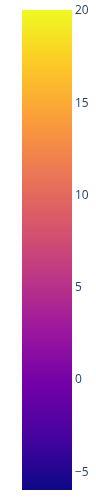
\includegraphics[height=3cm]{plots/Colorscales/Plasma.png}{Plasma}
% \caption{Colour scale for the 'Gained Points' surfaces}
% \label{fig:Plasma}
% \end{wrapfigure}
% In the following two pages, you will see all the surfaces of both Random-Discrete and Random-Continuous.
% There are five surfaces in each interaction that are generated from one ICPD.
% The x-axis, the one in be bottom-right, shows the parameter of the main strategy.
% The y-axis, the other axis on the bottom, indicates the parameter of the opponent.
% The z-axis always shows the points.
% All the surfaces are not only marked by height but also by colour.
% The context in which points are displayed depends on the surface. 
% The first two rows are the most basic surface plots.
% They show the gains of the strategy itself and the opponent's.
% The highest point that can appear is at 30.
% And the lowest is at 0.
% The maximum can be calculated by regarding the pay-off equations.
% The maximum points are gained by exploitation.
% So, $P_A =  y - c \cdot x + c$ becomes by substitution $P_A = 1 - 0.5 \cdot 0 + 0.5$ \textrightarrow $P_A = 1.5$.
% And since the CPD is played 20 times, $P_A \cdot 20 = 30$.
% So, the boundaries in which the points can vary is from 0 to 30.
% All the points, that are at height 20, have their correspondence in the other surface since in order to get 20 points, mutual cooperation is required.
% The same principle can be allied to the maximum, minimum points and mutual defection which is at height 10.
% Wherever a minimum point can be seen, the correspondence is the maximum point at the same x-y-coordinate.
% The colour of the points indicates the same as the height, the number of points.
% So, one can read this surface more accurately by regarding Figure \ref{fig:Plasma}.
% The next two surfaces concern the advantage one strategy has over the other.
% This shows us how much more one strategy had over the other.
% For the surface of the main strategy, simply the opponent's surface is subtracted from it's surface and vice versa.
% The maximum and the minimum can be calculated by taking the difference of the maximum and the minimum of the first two surfaces.
% So, the points can vary between -30 and 30.
% (30 - 0 = 30, 0 - 30 = -30)
% The two initial surfaces would intersect if they were put into one coordinate system.
% The intersection is at all the locations where the both strategies have gained an equal amount of points.
% At this location of the intersection, the surface plot, that demonstrates the advantage, would intersect with the zero-plane because the difference of two same number is always equal to zero.\\
% The two advantage surfaces are always mirrored by the zero-plane since every time you subtract $A-B$, it is the same as $(B-A) \cdot -1$.\\
% If this surface plot happens to be completely over the zero-plane, it means that the displays strategy has won every game they have played.
% Also here, there is a colour scale.
% This colour scale, however, differs from the first one.
% I chose to use different colour scales for visualisation purposes due to the fact that the advantage surfaces have a different z-axis range than the first two.
% (-30 to 30)
% B)
% % 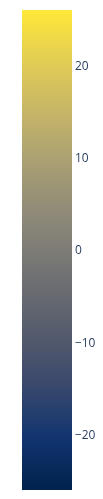
\includegraphics[height=3.0cm]{plots/Colorscales/Cividis.png}
% The last row of surfaces displays how much points have been gained by both.
% To generate these surfaces, one must add the surfaces which describe how much one has gained of the concerned strategies.
% Looking at the pay-off equations, a point can not be over the limit of 20.
% Both gain the most if both cooperate.
% Following the equations, one gets 1 point after every round.
% Since 20 rounds are played in total, the maximum is at 20.
% (20 rounds * 1 point = 20 points)
% I decided to also plot this surface to demonstrate the population welfare.
% This means that the higher the points, the most have gained both together.
% This plot has, as the advantage surfaces, a different z-axis range.
% So a new colour scale is introduced.
% C)
\newpage

% 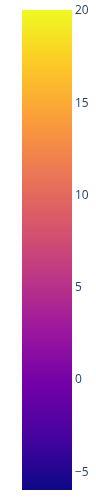
\includegraphics[height=3cm]{plots/Colorscales/Plasma.png}
% 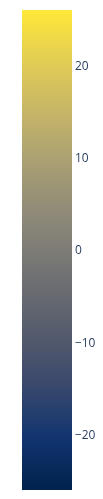
\includegraphics[height=3cm]{plots/Colorscales/Cividis.png}
% 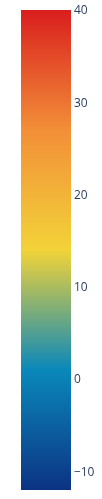
\includegraphics[height=3cm]{plots/Colorscales/Portland.png}

\newpage

\def\w{0.16}
\def\a{30}

% ------------------------------- Random-Discrete -------------------------------
\begin{figure}[h]
	\centering
    
	% Header row
	\begin{tabular}{p{0.7cm}ccccc}
		& \rotatebox{\a}{Random-Discrete} & \rotatebox{\a}{Random-Continuous} & \rotatebox{\a}{AlwaysSame} & \rotatebox{\a}{Adapt-Discrete} & \rotatebox{\a}{Adapt-Continuous} \\[1cm]
		
		% Gain Random-Discrete row
		\rotatebox{90}{\parbox{2cm}{\centering Gain \\ Random-Discrete}} &
		\includegraphics[width=\w\textwidth]{plots/Random-Discrete/Random-Discrete_vs_Random-Discrete_2/Random-Discrete.png} &
		\includegraphics[width=\w\textwidth]{plots/Random-Discrete/Random-Discrete_vs_Random-Continuous/Random-Discrete.png} &
		\includegraphics[width=\w\textwidth]{plots/Random-Discrete/Random-Discrete_vs_AlwaysSame/Random-Discrete.png} &
		\includegraphics[width=\w\textwidth]{plots/Random-Discrete/Random-Discrete_vs_Adapt-Discrete/Random-Discrete.png} &
		\includegraphics[width=\w\textwidth]{plots/Random-Discrete/Random-Discrete_vs_Adapt-Continuous/Random-Discrete.png} \\[0.5cm]
		
		% Gain Opponent row  
		\rotatebox{90}{\parbox{2cm}{\centering Gain \\ Opponent}} &
		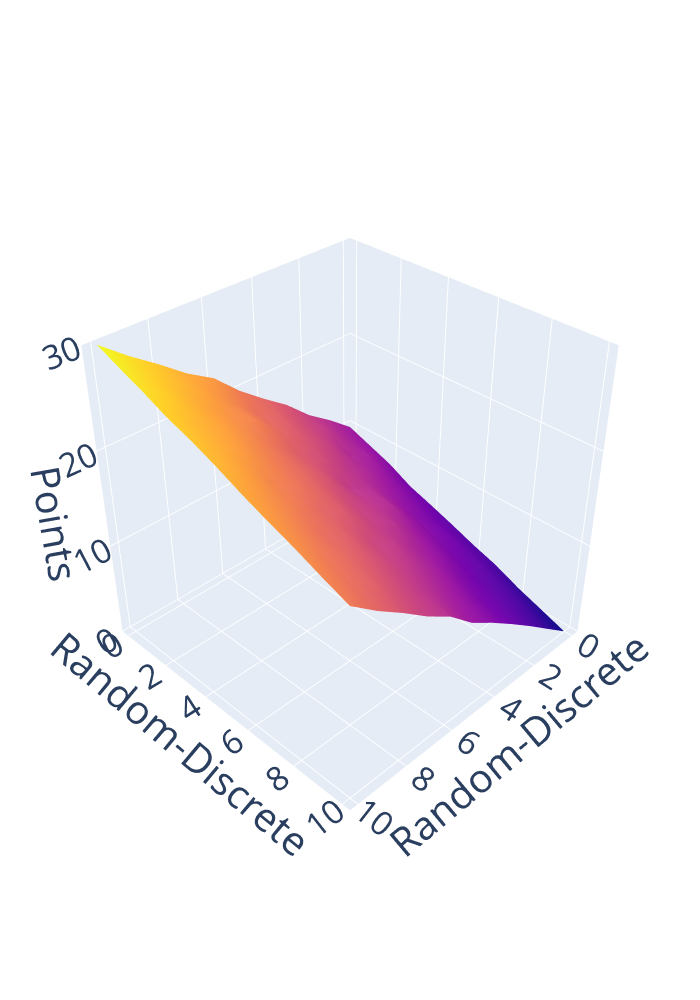
\includegraphics[width=\w\textwidth]{plots/Random-Discrete/Random-Discrete_vs_Random-Discrete_2/Random-Discrete_2.png} &
		\includegraphics[width=\w\textwidth]{plots/Random-Discrete/Random-Discrete_vs_Random-Continuous/Random-Continuous.png} &
		\includegraphics[width=\w\textwidth]{plots/Random-Discrete/Random-Discrete_vs_AlwaysSame/AlwaysSame.png} &
		\includegraphics[width=\w\textwidth]{plots/Random-Discrete/Random-Discrete_vs_Adapt-Discrete/Adapt-Discrete.png} &
		\includegraphics[width=\w\textwidth]{plots/Random-Discrete/Random-Discrete_vs_Adapt-Continuous/Adapt-Continuous.png} \\[0.5cm]
		
		% Advantage Random-Discrete row
		\rotatebox{90}{\parbox{2cm}{\centering Advantage \\ Random-Discrete}} &
		\includegraphics[width=\w\textwidth]{plots/Random-Discrete/Random-Discrete_vs_Random-Discrete_2/Random-Discrete_diff.png} &
		\includegraphics[width=\w\textwidth]{plots/Random-Discrete/Random-Discrete_vs_Random-Continuous/Random-Discrete_diff.png} &
		\includegraphics[width=\w\textwidth]{plots/Random-Discrete/Random-Discrete_vs_AlwaysSame/Random-Discrete_diff.png} &
		\includegraphics[width=\w\textwidth]{plots/Random-Discrete/Random-Discrete_vs_Adapt-Discrete/Random-Discrete_diff.png} &
		\includegraphics[width=\w\textwidth]{plots/Random-Discrete/Random-Discrete_vs_Adapt-Continuous/Random-Discrete_diff.png} \\[0.5cm]
		
		% Advantage Opponent row
		\rotatebox{90}{\parbox{2cm}{\centering Advantage \\ Opponent}} &
		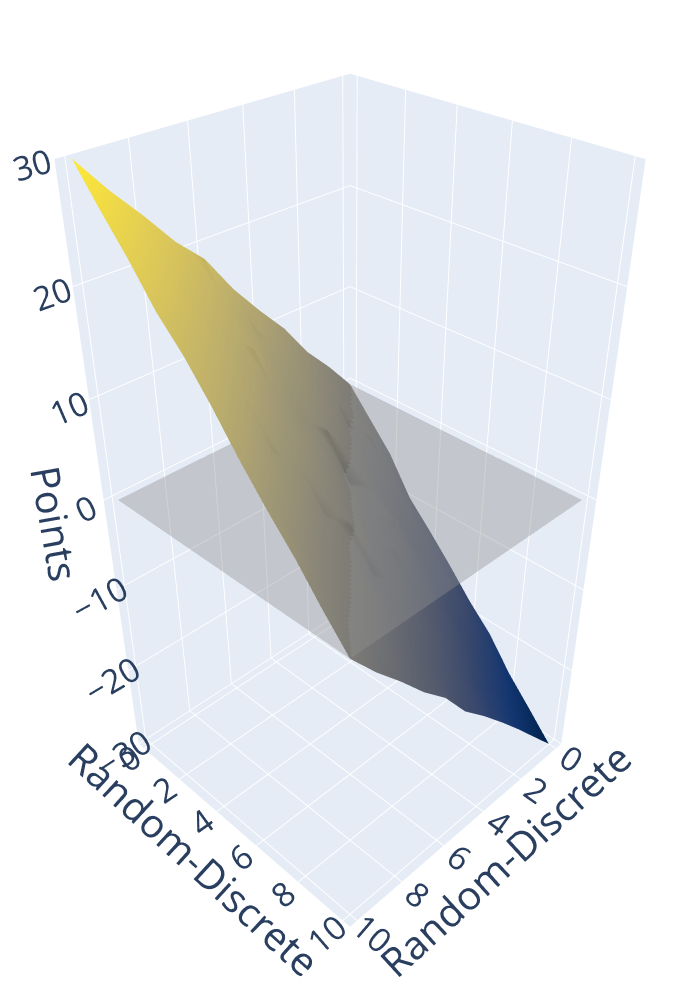
\includegraphics[width=\w\textwidth]{plots/Random-Discrete/Random-Discrete_vs_Random-Discrete_2/Random-Discrete_2_diff.png} &
		\includegraphics[width=\w\textwidth]{plots/Random-Discrete/Random-Discrete_vs_Random-Continuous/Random-Continuous_diff.png} &
		\includegraphics[width=\w\textwidth]{plots/Random-Discrete/Random-Discrete_vs_AlwaysSame/AlwaysSame_diff.png} &
		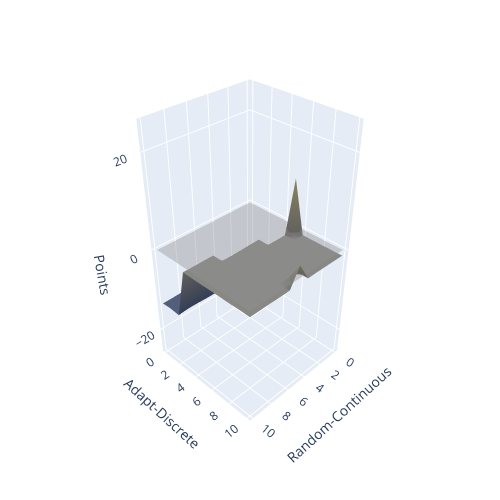
\includegraphics[width=\w\textwidth]{plots/Random-Discrete/Random-Discrete_vs_Adapt-Discrete/Adapt-Discrete_diff.png} &
		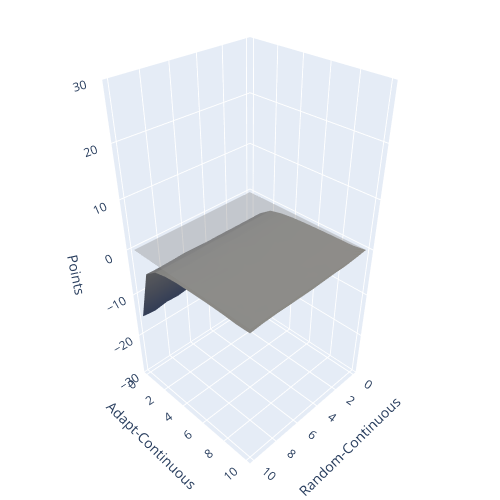
\includegraphics[width=\w\textwidth]{plots/Random-Discrete/Random-Discrete_vs_Adapt-Continuous/Adapt-Continuous_diff.png} \\[0.5cm]
		
		% Overall Gain row
		\rotatebox{90}{\parbox{2cm}{\centering Overall \\ Gain}} &
		\includegraphics[width=\w\textwidth]{plots/Random-Discrete/Random-Discrete_vs_Random-Discrete_2/added.png} &
		\includegraphics[width=\w\textwidth]{plots/Random-Discrete/Random-Discrete_vs_Random-Continuous/added.png} &
		\includegraphics[width=\w\textwidth]{plots/Random-Discrete/Random-Discrete_vs_AlwaysSame/added.png} &
		\includegraphics[width=\w\textwidth]{plots/Random-Discrete/Random-Discrete_vs_Adapt-Discrete/added.png} &
		\includegraphics[width=\w\textwidth]{plots/Random-Discrete/Random-Discrete_vs_Adapt-Continuous/added.png} \\
	\end{tabular}
	\caption{pbICPD of Random-Discrete.}
	\label{fig:RNDD-table}
\end{figure}

\newpage
% ------------------------------- Random-Continuous -------------------------------
\begin{figure}[h]
    \centering
    
	% Header row
	\begin{tabular}{p{0.7cm}ccccc}
		& \rotatebox{\a}{Random-Discrete} & \rotatebox{\a}{Random-Continuous} & \rotatebox{\a}{AlwaysSame} & \rotatebox{\a}{Adapt-Discrete} & \rotatebox{\a}{Adapt-Continuous} \\[1cm]
		
		% Gain Random-Continuous row
		\rotatebox{90}{\parbox{2cm}{\centering Gain \\ Random-Continuous}} &
		\includegraphics[width=\w\textwidth]{plots/Random-Continuous/Random-Continuous_vs_Random-Discrete/Random-Discrete.png} &
		\includegraphics[width=\w\textwidth]{plots/Random-Continuous/Random-Continuous_vs_Random-Continuous_2/Random-Continuous.png} &
		\includegraphics[width=\w\textwidth]{plots/Random-Continuous/Random-Continuous_vs_AlwaysSame/Random-Continuous.png} &
		\includegraphics[width=\w\textwidth]{plots/Random-Continuous/Random-Continuous_vs_Adapt-Discrete/Random-Continuous.png} &
		\includegraphics[width=\w\textwidth]{plots/Random-Continuous/Random-Continuous_vs_Adapt-Continuous/Random-Continuous.png} \\[0.5cm]
		
		% Gain Opponent row  
		\rotatebox{90}{\parbox{2cm}{\centering Gain \\ Opponent}} &
		\includegraphics[width=\w\textwidth]{plots/Random-Continuous/Random-Continuous_vs_Random-Discrete/Random-Continuous.png} &
		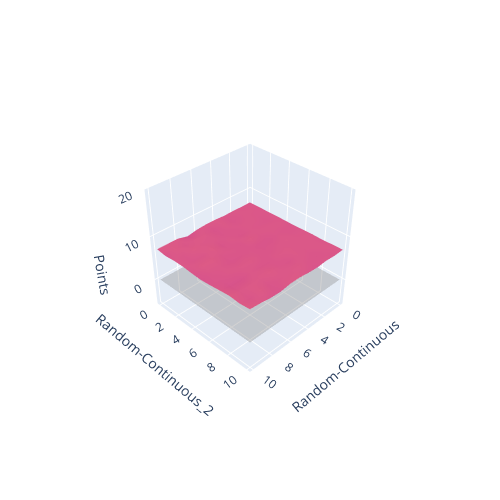
\includegraphics[width=\w\textwidth]{plots/Random-Continuous/Random-Continuous_vs_Random-Continuous_2/Random-Continuous_2.png} &
		\includegraphics[width=\w\textwidth]{plots/Random-Continuous/Random-Continuous_vs_AlwaysSame/AlwaysSame.png} &
		\includegraphics[width=\w\textwidth]{plots/Random-Continuous/Random-Continuous_vs_Adapt-Discrete/Adapt-Discrete.png} &
		\includegraphics[width=\w\textwidth]{plots/Random-Continuous/Random-Continuous_vs_Adapt-Continuous/Adapt-Continuous.png} \\[0.5cm]
		
		% Advantage Random-Continuous row
		\rotatebox{90}{\parbox{2cm}{\centering Advantage \\ Random-Continuous}} &
		\includegraphics[width=\w\textwidth]{plots/Random-Continuous/Random-Continuous_vs_Random-Discrete/Random-Continuous_diff.png} &
		\includegraphics[width=\w\textwidth]{plots/Random-Continuous/Random-Continuous_vs_Random-Continuous_2/Random-Continuous_diff.png} &
		\includegraphics[width=\w\textwidth]{plots/Random-Continuous/Random-Continuous_vs_AlwaysSame/Random-Continuous_diff.png} &
		\includegraphics[width=\w\textwidth]{plots/Random-Continuous/Random-Continuous_vs_Adapt-Discrete/Random-Continuous_diff.png} &
		\includegraphics[width=\w\textwidth]{plots/Random-Continuous/Random-Continuous_vs_Adapt-Continuous/Random-Continuous_diff.png} \\[0.5cm]
		
		% Advantage Opponent row
		\rotatebox{90}{\parbox{2cm}{\centering Advantage \\ Opponent}} &
		\includegraphics[width=\w\textwidth]{plots/Random-Continuous/Random-Continuous_vs_Random-Discrete/Random-Discrete_diff.png} &
		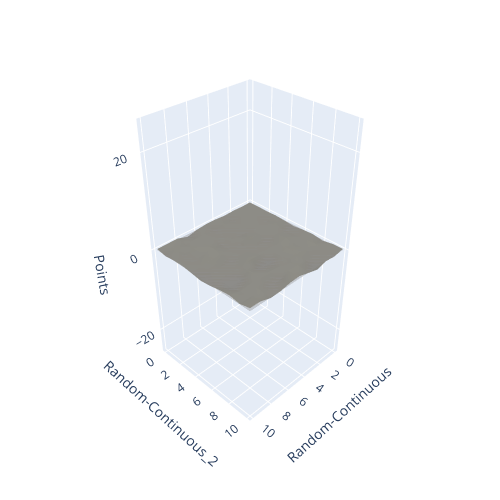
\includegraphics[width=\w\textwidth]{plots/Random-Continuous/Random-Continuous_vs_Random-Continuous_2/Random-Continuous_2_diff.png} &
		\includegraphics[width=\w\textwidth]{plots/Random-Continuous/Random-Continuous_vs_AlwaysSame/AlwaysSame_diff.png} &
		\includegraphics[width=\w\textwidth]{plots/Random-Continuous/Random-Continuous_vs_Adapt-Discrete/Adapt-Discrete_diff.png} &
		\includegraphics[width=\w\textwidth]{plots/Random-Continuous/Random-Continuous_vs_Adapt-Continuous/Adapt-Continuous_diff.png} \\[0.5cm]
		
		% Overall Gain row
		\rotatebox{90}{\parbox{2cm}{\centering Overall \\ Gain}} &
		\includegraphics[width=\w\textwidth]{plots/Random-Continuous/Random-Continuous_vs_Random-Discrete/added.png} &
		\includegraphics[width=\w\textwidth]{plots/Random-Continuous/Random-Continuous_vs_Random-Continuous_2/added.png} &
		\includegraphics[width=\w\textwidth]{plots/Random-Continuous/Random-Continuous_vs_AlwaysSame/added.png} &
		\includegraphics[width=\w\textwidth]{plots/Random-Continuous/Random-Continuous_vs_Adapt-Discrete/added.png} &
		\includegraphics[width=\w\textwidth]{plots/Random-Continuous/Random-Continuous_vs_Adapt-Continuous/added.png} \\
	\end{tabular}
	\caption{pbICPD of Random-Continuous.}
	\label{fig:RNDC-table}
\end{figure}

\newpage

In the following two pages, the results of each column, meaning the five surface plots, will be presented objectively.
The description of each interaction follows a certain pattern. 
First, the two absolute-gain surfaces are exhibited.
Second, both relative-gain surface plots are explained.
Ultimately, the overall-gain surface is clarified.\\

\subsection{Random-Discrete}

\subsubsection*{Random-Discrete\textunderscore2}
		The left (10, 0) and right (0, 10) corner are the extremes.
		Random-Discrete is exploited if its parameter is equal to 10, meaning it corresponds to AlwaysCooperate, and Random-Discrete\textunderscore2's parameter is at 0, i.e. it is equivalent to AlwaysDefect.
		% This is how one can get the maximum output, by exploiting.
		% This can be seen in the surface of Random-Discrete\textunderscore2.
		The hindmost corner at the coordinate (0, 0) is where both defect constantly.
		This fact can be excogitated by the bespoken feature that this coordinate is located at a z-coordinate of 10.
		% This is the point where both get their relative lowest output, as can be seen later.\\
		The nearest point to this perspective is at the coordinate (10, 10).
		Either's value of their parameter is 10, this indicates that both Random-Discrete and Random-Discrete\textunderscore2 behave equally, viz. as AlwaysCooperate.
		So, both always cooperate and thus gain 20 points separately.\\

		The peaks of both relative-gain surface plots derive from having the maximum output.
		Since one can get the maximum output only if the other is exploited, the advantage surface result in the highest z-value possible.
		When the two parameter's are identical, however, they are not any better than the other.
		This makes sense since they behave the same when they have the same parameter and can thus not exploit each other.\\

		The overall-gain surface indicates clearly that the pinnacle of the slope is at (10, 10).
		This point, as already mentioned, has the quality that both strategies are equal to AlwaysCooperate.
		% This illustrates the dilemma pretty well.
		On the opposite corner, however, it becomes clear this is the lowest point.
		As already mentioned, the most behind point, being the lowest, results from the fact that both defected constantly.
		So, for the welfare of the population, it is best if both cooperate interminably.\\


\subsubsection*{Random-Continuous}
		The absolute-gain surfaces concerning the interaction of Random-Discrete and Random-Continuous range from 20 to 10 and from 5 to 25 continuously.
		Both surfaces are not influenced by the parameter of Random-Continuous.\\
		% This is logical and will be looked at the discussion.\\

		The two relative-gain surfaces, if put together in one plot, would intersect exactly in the middle where the parameter of Random-Discrete is equal to 5.
		Since they range from different limits but both upper and lower limit add up to 30, they intersect in the middle where the parameter of Random-Discrete is 5.
		That is why the surface of the relative-gain intersects the zero-plane at the same line.
		Naturally, this surface is only influenced by the parameter of Random-Discrete and not Random-Continuous.
		They range continuously from -15 to 15.\\

		The overall-gain surface shows a constant slope ranging from 35 to 25.
		The maximum value, 40, has not been achieved since exploitation did not take place.\\


\subsubsection*{AlwaysSame}
		It has to be mentioned that Random-Discrete behaves like AlwaysSame.
		This is due to the fact that this simulation has been run 100 times to smooth out one-time abnormalities.
		This is notable by looking at the column where Random-Discrete plays against itself and against AlwaysSame.
		Since the two strategies behave exactly in the same way, these two columns of surface plots are duplicates.
		The differential between Random-Discrete and AlwaysSame is later defined in the Discussion.\\


\subsubsection*{Adapt-Discrete}
		In the surface of Random-Discrete against Adapt-Discrete, there is a stripe at the parameter of Adapt-Discrete being from 0 to 2.
		This stripe ranges from absolute exploitation at (0, 0) to mutual cooperation at parameter of Random-Discrete being equal to 10.
		Abruptly, this stripe does not follow its pattern in the y-direction any more.
		Rather a new inclination is visible.
		This sudden alternation will be analysed in the Discussion. 
		This slope's lowest points are at a height of 10.
		But, both slopes range from where they begin at the y-z-plane to 20 at the other y-z-plane.
		Respecting the fact that the height of 20 is an indicator of mutual cooperation, it can be verified by regarding the height of the correspondent points.
		Since they are indeed at the same height, mutual cooperation takes place where the parameter of Random-Discrete is equal to 10.
		Also the maximum points of the first plot indicate that the same points on the other surface must be at height 0.\\
		% The broader slope is also going downwards.
		% But this slope is not as steep as the one on the other surface and thus has lower points at the edge where the parameter of Random-Discrete is 0.
		% When Random-Discrete has its parameter at 10, which means it behaves like AlwaysCooperate, mutual cooperation will take place.\\

		The relative-gain surface of Adapt-Discrete hides its most interesting element, the inverted stripe that leads ends at absolute exploitation and thus at height 0.
		The rest of the surface is very near to the zero-plane which means it was as good as Random-Continuous in this area.
		Because the slopes look pretty similar, there are practically no advantages in this scope.
		At the coordinates of the stripe, however, is a great advantage which only Random-Continuous has over Adapt-Discrete.\\

		As a matter of course, the overall-gain surface is the highest where only mutual cooperation occurred, which is where the parameter of Random-Discrete is equal to 10.
		The stripe breaks off at height 30 which indicates exploitation.
		And the broader slope finishes at height 20 which suggests mutual defection.\\


\subsubsection*{Adapt-Continuous}
		The absolute-gain surfaces look akin to the ones against Adapt-Discrete.
		The difference concerns the angularity.
		Curves appear to replace the edges.\\
		Since this phenomenon differs from that in the interaction between Adapt-Discrete, also this occurrence will be investigated further in the Discussion.
		
		% The edge where points are at height 20, stays as it was in the game against Adapt-Discrete.
		% The broad slope is also similar to that surface, its lowest points being at 10.
		% The surface of Adapt-Continuous is in a same way similar to the one of Adapt-Discrete.
		% The edges are curved out.
		% But, the slope is, again, a bit steeper than the one of Random-Discrete.\\

		The same applies to the relative-gain and overall-gain surface plots.\\

		% The advantage surface of Adapt-Continuous is in a difficult angle to see.
		% The origin of the coordinate-system is the lowest point of this surface.
		% I concluded this fact by knowing that the highest point of the other advantage surface has its correspondence at height 0.\\
		%
		% The maximum points are aligned in a line.
		% More specific, an edge of the surface at height 40.
		% The least points are gained at the edge more behind at the y-z-plane.
		% This edge is rather a curve than a straight line.
		% This curve bows from exploitation at coordinates being at (0, 0) to 20, the absolute minimum of this surface.
	
\subsection{Random-Continuous}

\subsubsection*{Random-Discrete}
		Certain interactions appear twice, as this one.
		Random-Discrete has already played against Random-Continuous.
		There is thus no need for any explanation.\\
	

\subsubsection*{Random-Continuous\textunderscore2}
		As already mentioned, Random-Continuous behaves like AlwaysNeutral by having played several times.
		This results to having a completely flat surface.
		We can calculate at which height the surface is.
		Plugging in 0.5 for both $x$ and $y$ in the pay-off equations, we get $P_A = 0.5 - c \cdot 0.5 + c$ where $c = 0.5$.
		The pay-off of strategy A is $P_A = 0.75$ and having played the ICPD 20 rounds, it is equal to $P_A \cdot 20 = 15$.
		Both strategies A and B get the same pay-off since they submitted the same investment.
		$P_B = P_A \rightarrow P_B \cdot 20 = 15$.
		So, both surfaces are at the same height at every point.\\

		Subtracting two flat surfaces at the same height at every coordinate, results in an also flat surface which corresponds to the zero-plane.
		No strategy was better than the other at any point.\\

		Adding these even two surfaces which are both at height 15, a surface at height $15 + 15 = 30$ follows.\\


\subsubsection*{AlwaysSame}
		These surfaces are identical to the one's of the Random-Continuous vs. Random-Discrete interaction.
		I will not describe them as they already have been.\\
	

\subsubsection*{Adapt-Discrete}
		There are two main levels on this surface.
		The upper level in the Random-Continuous surface is at z-coordinate equal to 25 and lower to 10.
		There is a little peak at the coordinate (5, 10) with an approximate height of 17, 12 respectively.\\
		It seems as if the two absolute-gain surfaces are congruent.
		This lower level is at $z = 10$ and the upper one at $z = 15$.
		Also, the peak is pointing downwards making it to a lacuna.\\

		The upper level of the absolute-gain surface of Random-Continuous is approximately 15 points higher than the lower level of the other absolute-gain plot.
		Additionally, the lower level of the surface of Random-Continuous and the upper one of the surface of Adapt-Discrete have nearly the same z component.
		Notably, the relative-gain surface of Random-Continuous is above the zero-plane.
		This means that Random-Continuous was better in every single game.\\

		According to this surface, the upper level of the absolute-gain surface of Random-Continuous added to the lower level of the one of Adapt-Discrete is greater than adding the two other levels.
		The peak pointing upwards indicates that the peak is higher than the lacuna is profound.\\
		

\subsubsection*{Adapt-Continuous}
		The absolute-gain surfaces resemble a wave or a curve in the y-direction.
		This derives from the fact that, as already mentioned, Random-Continuous behaves like AlwaysNeutral.\\
		The upper and lower limits conform to that of the correspondent absolute-gain surfaces against Adapt-Discrete.
		Interestingly, this curve gives the impression that the lower limit has been reached once the parameter of Adapt-Continuous arrives at a certain value, estimative 4.

		The same properties can be seen in the relative-gain surface plots.
		Upper and lower limits correspond to that of the relative-gain surfaces against Adapt-Discrete.
		Also, the relative-gain surface of Random-Continuous is completely above the zero-plane.\\

		This bespoken relation between the interaction against Adapt-Discrete is indifferent in the overall-gain surface plot.
		The upper limit is at $z = 35$ and the lower boundary is at z-coordinate equal to 30.


\section{Discussion}

The results suggest certain effects of the PD.
Many additional findings have been identified and were promised to be analysed in the Discussion since they need mathematical context for better understanding.

\subsection{Shallow Randomness} \label{sec:shallow_randomness}

	% TODO: Explain what a mixed strategy is in foundations
	Random-Discrete and Random-Continuous, as a mixed strategies, behave equitably as pure strategies if the average of all the generated surfaces is taken.
	The mathematical framework used to describe this phenomenon is called the Law of Large Numbers (LLN).
	100 repetitions were named to be sufficient.
	Random-Discrete acts identically as AlwaysSame and Random-Continuous as AlwaysNeutral.

\subsubsection*{Random-Discrete}
		
	To clarify the resemblance between Random-Discrete and AlwaysSame, the equations to calculate the investment have to analysed.
	\begin{equation}
		\begin{split}
		% \Pr(i = 1 \mid \theta_{\mathrm{RndD}}) = \frac{\theta_{\mathrm{RndD}}}{10}
		% \text{ or }
		% i \;\sim\; \mathrm{Bernoulli}(\frac{\theta_{\mathrm{RndD}}}{10})\\
		i \;\sim\;
		\begin{cases}
		  1 & \text{with probability } \frac{1}{2}\\
		 -1 & \text{with probability } \frac{1}{2} 
		\end{cases}
		\label{eq:RNDD_i_eq}
		\end{split}
	\end{equation}

	Regarding the investment calculation of Random-Discrete (\ref{eq:RNDD_i_eq}), we can generate $n$ $i$'s (\ref{eq:RNDD_n_i}).

	\begin{equation}
		i_1, i_2, i_3, \dots, i_n \;\sim \mathrm{Bernoulli}(\frac{\theta_{\mathrm{RndD}}}{10})
		\label{eq:RNDD_n_i}
	\end{equation}

	\begin{equation}
		\begin{split}
			\lim_{n\to\infty} \frac{1}{n} \sum_{k=1}^{n} i_k &= \frac{\theta_{\mathrm{RndD}}}{10} \text{ almost surely}\\
			\frac{1}{100} \sum_{k=1}^{100} i_k &\approx \frac{\theta_{\mathrm{RndD}}}{10}
		\label{eq:RNDD_approx_eq}
		\end{split}
	\end{equation}

	Substituting $n$ with 100 in equation (\ref{eq:RNDD_approx_eq}) would be an approximation.
	But, for the scope of this project, 100 repetitions were named to be sufficient.\\
	The fact that the surfaces of AlwaysSame seem identical to those against itself is now proven and justified.
	
\subsubsection*{Random-Continuous}

	Also in this case, the investment calculations need to be investigated to understand the appearance of AlwaysNeutral.

	\begin{equation}
		i(\theta_{\mathrm{RndC}}) = 0.5 + s(\theta_{\mathrm{RndC}})
		\label{eq:RNDC_i_eq}
	\end{equation}
	\begin{equation}
		s(\theta_{\mathrm{RndC}}) = \epsilon \cdot \frac{\theta_{\mathrm{RndC}}}{20}
		\label{eq:RNDC_s_eq}
	\end{equation}
	\begin{equation}
		\begin{split}
		% \Pr(\epsilon = 1) = \Pr(\epsilon = -1) = \frac{1}{2} \text{ or } \epsilon \;\sim 2 \cdot \mathrm{Bernoulli}(\frac{1}{2}) - 1\\
		\epsilon \;\sim\;
		\begin{cases}
		  1 & \text{with probability } \frac{1}{2}\\
		 -1 & \text{with probability } \frac{1}{2} 
		\end{cases}
		\label{eq:prob_eps}
		\end{split}
	\end{equation}

	Only the equation (\ref{eq:RNDC_s_eq}) is considerable since the probability or randomness singly appears there.
	The same procedure is applied.

	\begin{equation}
		% \epsilon_1, \epsilon_2, \epsilon_3, \dots, \epsilon_n \;\sim 2 \cdot \mathrm{Bernoulli}(\frac{1}{2}) - 1
		\epsilon_1, \epsilon_2, \epsilon_3, \dots, \epsilon_n \;\sim\; 
		\begin{cases}
		  1 & \text{with probability } \frac{1}{2}\\
		 -1 & \text{with probability } \frac{1}{2} 
		\end{cases}
		\label{eq:RNDC_n_i}
	\end{equation}
	\begin{equation}
		\begin{split}
			\lim_{n\to\infty} \frac{1}{n} \sum_{k=1}^{n} \epsilon_k &= 0 \text{ almost surely}\\
			\bar \epsilon = \frac{1}{100} \sum_{k=1}^{100} \epsilon_k &\approx 0
		\label{eq:RNDC_approx_eq}
		\end{split}
	\end{equation}

	As a consequence of that, the investment is always equal to 0.5, as shows equation (\ref{eq:i_eq_0.5}).

	\begin{equation}
		\begin{split}
			i(\theta_{\mathrm{RndC}}) = 0.5 + \bar \epsilon \cdot \frac{\theta_{\mathrm{RndC}}}{20} = 0.5
		\end{split}
		\label{eq:i_eq_0.5}
	\end{equation}

	The non-existent influence of Random-Continuous' parameter is traced back to this fact.


\subsection{Random-Discrete vs. AlwaysSame} \label{sec:RndD_vs_AlwS}
	
	Random-Discrete, as a mixed strategy, behaves equitably as AlwaysSame when taking the average of all the generated surfaces.
	In the simulation, all games were played 100 times and taken the average.
	Having the surface only generated once, results in a different-looking surface as Figure \ref{fig:two_one-iter} reveals.\\

	\begin{figure}[h]
		\centering
		\begin{subfigure}[t]{0.45\textwidth}
			\centering
			\includegraphics[width=\linewidth]{plots/Discussion/Random-Discrete_vs_AlwaysSame/Random-Discrete_first.png}
			\caption{Absolute-gain surface of Random-Discrete.}
			\label{fig:RNDD_one-iter}
		\end{subfigure}\hfill
		\begin{subfigure}[t]{0.45\textwidth}
			\centering
			\includegraphics[width=\linewidth]{plots/Discussion/Random-Discrete_vs_AlwaysSame/AlwaysSame_first.png}\\
			\caption{Absolute-gain surface of AlwaysSame.}
			\label{fig:ALWS_one-iter}
		\end{subfigure}
		\caption{One iteration of the pbICPD.}
		\label{fig:two_one-iter}
	\end{figure}

	Figure \ref{fig:RNDD_one-iter} and \ref{fig:ALWS_one-iter} show the gained points of Random-Discrete and AlwaysSame when playing the pbICPD solely once.
	A more coarse surface is visible.
	This joltiness is due to the fact that Random-Discrete uses probabilities after all.
	Where as AlwaysSame submits always a determined investment.\\
	The surface of Random-Discrete is a bit evener. 
	This fact can be explained by examining the pay-off equations:
	$P_A = y - c \cdot x + c$ and $P_B = x - c \cdot y + c$\\
	$x$ being the previous investment of Random-Discrete and $y$ is equal to the previous investment of AlwaysSame.
	$x$ is relatively random, depending on Random-Discrete's parameter and $y$ is a constant over one game.
	Subtracting only a fraction of the random investment pays off a more constant amount of points.\\
	To calculate how much Random-Discrete digresses from its constant-behavioured opponent, we can use the standard deviation for every game.
	This means we can display a new surface plot which will describe the deviation of the investments compared to the average.
	Using equation (\ref{eq:standard_deviation}), the Standard Deviation (SD), Figures \ref{fig:RNDD_one-iter} and \ref{fig:ALWS_one-iter} are generated.
	\begin{equation}
		s = \sqrt{\frac{1}{N-1} \sum_{i=1}^N (x_i - \overline{x})^2}
		\label{eq:standard_deviation}
	\end{equation}
	\begin{figure}[h]
		\centering
		\begin{subfigure}[t]{0.45\textwidth}
			\centering
				\includegraphics[width=\linewidth]{plots/Discussion/Random-Discrete_vs_AlwaysSame/Random-Discrete_sd.png}
			\caption{Standard Deviation surface of Random-Discrete.}
			\label{fig:RNDD_one-iter}
		\end{subfigure}\hfill
		\begin{subfigure}[t]{0.45\textwidth}
			\centering
				\includegraphics[width=\linewidth]{plots/Discussion/Random-Discrete_vs_AlwaysSame/AlwaysSame_sd.png}
			\caption{Standard Deviation surface of AlwaysSame.}
			\label{fig:ALWS_one-iter}
		\end{subfigure}
		\caption{Standard Deviation surfaces.}
		\label{fig:two_one-iter}
	\end{figure}
	To conclude, choosing AlwaysSame, especially parameter from 2 to 8, as one's own behaviour means a high risk of loosing or winning as shows Figure \ref{fig:ALWS_one-iter}.
	This deviation from the average is at every point twice as much with AlwaysSame than Random-Discrete.

	This can be seen in these two following surface plots.
	\begin{figure}[h]
		\centering
		\begin{subfigure}[t]{0.45\textwidth}
			\centering
				\includegraphics[width=\linewidth]{plots/Discussion/Random-Discrete_vs_AlwaysSame/Random-Discrete_sd_p_avr.png}
			\caption{Standard Deviation $\pm$ Average surface of Random-Discrete.}
			\label{fig:RNDD_sd_pm_avr}
		\end{subfigure}\hfill
		\begin{subfigure}[t]{0.45\textwidth}
			\centering
				\includegraphics[width=\linewidth]{plots/Discussion/Random-Discrete_vs_AlwaysSame/AlwaysSame_sd_p_avr.png}
			\caption{Standard Deviation $\pm$ Average surface of AlwaysSame.}
			\label{fig:ALWS_sd_pm_avr}
		\end{subfigure}
		\caption{Standard Deviation $\pm$ Average surfaces.}
		\label{fig:Standard Deviation average.}
	\end{figure}

	The SD defines the boundaries in which 68.2\% of the samples lie within.
	So, the chance of getting a pay-off within this volume is equal to 68.2\%.\\
	Remarkably, the probability of loosing or winning is higher with AlwaysSame than Random-Discrete.
	This means that the Random-Discrete' pay-offs are more foreseeable than those of AlwaysSame.

\subsection{Random-Discrete vs. Adapt-Discrete} \label{sec:RndD_vs_AdpD}
		Glancing at the surface against Adapt-Discrete, this stripe is remarkable.
		The existence of this stripe and the factor of Adapt-Discrete's parameter from range 0 to 2 are clarified.\\
	\begin{equation}
		i(\theta_{\mathrm{AdpD}}) \;\sim\;
		\begin{cases}
			1 \text{ if } i_1 + s(\theta_{\mathrm{AdpD}}) \ge 0.5\\
			0 \text{ if } i_1 + s(\theta_{\mathrm{AdpD}}) < 0.5\\
		\end{cases}
		\label{eq:AdpD_rounded}
	\end{equation}

% $$i(\theta_{\mathrm{AdpD}}) = \round{i_1 + s(\theta_{\mathrm{AdpD}})}$$
	\begin{equation}
		s(\theta_{\mathrm{AdpD}}) = \frac{\theta_{\mathrm{AdpD}}}{5} \cdot (\bar i_1 - i_1)
		\label{eq:AdpD_eq_s}
	\end{equation}

	As Adapt-Discrete is defined, its investment is rounded to the nearest integer as expression (\ref{eq:AdpD_rounded}) demonstrates.
	To get from investment 0 to 1 or vice versa, its investment has to get over a certain threshold being equal to 0.5.
	In the first round, Adapt-Discrete contributes a 1.
	I.e. to surpass the threshold, $s(\theta_{\mathrm{AdpD}})$ must be under -0.5.
	To calculate a general formula that calculates the opponent's investment that is necessary to exceed the threshold in the first round given the parameter, it is required to solve for $\bar i_1$.

	\begin{alignat*}{2}
		s(\theta_{\mathrm{AdpD}}) &< -0.5 &&\\
		\frac{\theta_{\mathrm{AdpD}}}{5} \cdot (\bar i_1 - 1) &< -0.5 &&\qquad | \cdot \frac{5}{\theta_{\mathrm{AdpD}}} \\
		\bar i_1 - 1 &< -\frac{2.5}{\theta_{\mathrm{AdpD}}} &&\qquad | + 1 \\
		\bar i_1 &< -\frac{2.5}{\theta_{\mathrm{AdpD}}} + 1 &&
	\end{alignat*}

	Figure (\ref{fig:surpass_theshold_abs}) exhibits this the graph of this formula.
	The curve of this figure defines the area under it.
	Every point on this curve is not included.
	It implies every possible investment of the opponent in order Adapt-Discrete to surpass the threshold.
	\begin{figure}[h]
		\begin{center}
			\includegraphics[width=0.5\textwidth]{plots/Discussion/Adapt-Discrete/Adapt-Discrete_values_surpass_threshold_abs.png}
		\end{center}
		\caption{he}
		\label{fig:surpass_theshold_abs}
	\end{figure}

	It can be seen that the opponent's investment must be below zero to pass over the threshold value if $0 \le \theta_{\mathrm{AdpD}} \le 2$.
	A contribution below 0 is impossible.
	To conclude, if Adapt-Discrete's parameter is either 0, 1, or 2, the shift required to overstep the marginal value cannot be achieved.
	Thus, Adapt-Discrete is equivalent to AlwaysCooperate in cases where its parameter is equal to 0, 1, or 2.\\
	This explains the gainfulness of this stripe in the absolute-gain surface of Random-Discrete and thus the detriment of that stripe in the other absolute-gain surface.
	Adapt-Discrete is exploited since it cannot react because it only submits full cooperation in this area of the surface.\\

	Coming to the next attribute of this plot; the evenness of the rest of the surface.
	The other part of the surface is first, not influenced by the parameter of Adapt-Discrete and second, has a little inclination.
	The first point can be answered with the already proven fact that Random-Discrete parallels AlwaysSame.
	Adapt-Discrete mimics the opposing strategy if it belongs to the rigid category since the shift is equal to zero after the first few round, as will be discussed later.% explanation needed??
	\\
	The second quality can be justified by becoming clear about the fact that Random-Discrete will range its contributions from 0 to 1 as its parameter increases.
	But, a little detail can be observed concerning the inclinations of the two areas which do not coincide with each other.
	The subarea of the absolute-gain surface of Adapt-Discrete is a smidgen steeper than the other.
	This item substantiated by reason.
	Adapt-Discrete's first investment is always full cooperation.
	Random-Discrete with its parameter set to 0 acts like AlwaysDefect.
	Adapt-Discrete is thus completely exploited in the first round.
	Random-Discrete's parameter equal to 10, in contrary, will let Random-Discrete act like AlwaysCooperate.
	Hence, Adapt-Discrete is not at all exploited in the first round, and will never be during the game.
	To deduce, the nearer Random-Discrete's parameter is to zero, the more Adapt-Discrete is exploited in the first round.
	As a consequence of that, Adapt-Discrete will have a minor point deficit at most of the games.

\subsection{Random-Discrete vs. Adapt-Continuous}
	A same idea can be used to explain the similar appearance of the surfaces against Adapt-Continuous compared to the ones against Adapt-Discrete.
	The following line chart demonstrates the investments of Adapt-Continuous in one ICPD.
	I assumed that Random-Discrete behaves exactly the same as AlwaysSame due to discussed reasons (see sections \ref{sec:shallow_randomness} and \ref{sec:RndD_vs_AlwS}).
	Adapt-Continuous pursuits getting on the same level of investment as the opponent.\\
	Random-Discrete's parameter equals 5 in Figure \ref{fig:AdpC_approx_invetm_and_payoffs_0-5}.\\
	% AlwaysSame vs Adapt-Continuous better?
	\begin{figure}[h!]
		\centering
		\begin{subfigure}[t]{0.45\textwidth}
			\centering
			\includegraphics[width=\linewidth]{plots/Discussion/Adapt-Continuous/Approx_5_line_chart_0-5.png}\\
			\caption{Investments of Adapt-Continuous with parameters ranging from 0 to 5.}
			\label{fig:AdpC_approx_investm_0-5}
		\end{subfigure}
		\hfill
		\begin{subfigure}[t]{0.45\textwidth}
			\centering
			\includegraphics[width=\linewidth]{plots/Discussion/Adapt-Continuous/Approx_pay-offs_5_line_chart_0-5.png}
			\caption{Pay-offs of Adapt-Continuous with parameters ranging from 0 to 5.}
			\label{fig:AdpC_approx_payoff_0-5}
		\end{subfigure}
		\caption{}
		\label{fig:AdpC_approx_invetm_and_payoffs_0-5}
	\end{figure}

	The function to calculate each graph can be derived from the equation of Adapt-Continuous that calculates the investment.
	Equation (\ref{eq:AdpC_i_eq_rec}) describes this process recursively.
	$k$ indicates the current round and $\theta$ is the parameter of Adapt-Continuous.
	$\bar i$ has no numbering because it is constant.
	\begin{equation}
		i_k = i_{k-1} + \frac{\theta}{5} \cdot (\bar i - i_{k-1})
		\label{eq:AdpC_i_eq_rec}
	\end{equation}

	% derivation in appendix (ChatGPT)
	It is not possible to calculate a graph with the recursive form of this equation.
	The explicit version is required as equation (\ref{eq:AdpC_i_eq_expl}) implies.

	\begin{equation}
		i_k = \bar i + (1 - \frac{\theta}{5})^k \cdot (i_0 - \bar i)
		\label{eq:AdpC_i_eq_expl}
	\end{equation}
	
	The higher the parameter of Adapt-Continuous, the faster it can adjust its investment.
	This means that Adapt-Continuous, when the parameter is small, will be more exploited in the first several rounds than a Adapt-Continuous with a big value of its parameter.\\
	
	The question arises what the behaviour looks like if Adapt-Continuous' parameter has a value over 5.
	Figure \ref{fig:AdpC_approx_investm_5-10} demonstrates the answer to this question.\\
	\begin{figure}[h!]
		\centering
		\begin{subfigure}[t]{0.45\textwidth}
			\centering
			\includegraphics[width=\linewidth]{plots/Discussion/Adapt-Continuous/Approx_5_line_chart_5-10.png}
			\caption{Investments of Adapt-Continuous with parameters ranging from 5 to 10.}
			\label{fig:AdpC_approx_investm_5-10}
		\end{subfigure}
		\hfill
		\begin{subfigure}[t]{0.45\textwidth}
			\centering
			\includegraphics[width=\linewidth]{plots/Discussion/Adapt-Continuous/Approx_pay-offs_5_line_chart_5-10.png}
			\caption{Pay-offs of Adapt-Continuous with parameters ranging from 5 to 10.}
			\label{fig:AdpC_approx_payoff_5-10}
		\end{subfigure}
		\caption{}
		\label{fig:AdpC_approx_invetm_and_payoffs_5-10}
	\end{figure}
	
	The investments always overstep the value of the opponent's investment.
	The lines of parameters from six to nine tend to that value.
	The ultimate accumulated points they receive is, however, indifferent to that of the behaviour of parameter equal to ten.
	This is a consequence of the fact that the pay-offs of these investments cancel out.
	The points that are gained more is the counterpart of the deficit of points in the next round.
	
	The peaks and the lows at parameter from 5 to 10 converge into a common average.
	This average can be seen in Figure \ref{fig:AdpC_avr_points}.\\
	\begin{figure}[h]
		\begin{center}
			\includegraphics[width=0.5\textwidth]{plots/Discussion/Adapt-Continuous/payoffs_5_line_chart_0-10.png}
		\end{center}
		\caption{Accumulated points of Adapt-Continuous. Parameters ranging from 0 to 10.}
		\label{fig:AdpC_avr_points}
	\end{figure}
	
	To summarise, if $0 \le \theta \le 5$, their investment converge to the opponent's contribution since they can adapt faster the higher the parameter.
	If $5 \le \theta \le 10$ however, the investments equal the opponent's contribution since their overpassing the value of the opponent's investment results in an average being equal to the opponent's investment.\\
\subsection{Random-Continuous vs. Adapt-Discrete}
	The existence of two different plateaus is noteworthy.
	% \begin{figure}
	% 	\begin{center}
	% 		\includegraphics[width=0.5\textwidth]{plots/Discussion/Random-Continuous_vs_Adapt-Discrete/surface_2D.png}
	% 	\end{center}
	% 	\caption{}
	% 	\label{fig:AdpD_2D_surface}
	% \end{figure}
	
	Figures \ref{fig:RndC_investm} and \ref{fig:AdpD_surpass_threshold_infl_RndC} attempt to justify this attribute of the absolute-gain surface of Random-Continuous and Adapt-Continuous.
	\begin{figure}[h]
		\begin{center}
			\includegraphics[width=0.5\textwidth]{plots/Discussion/Random-Continuous/investments.png}
		\end{center}
		\caption{Investments of Random-Continuous. Parameters from 0 to 10.}
		\label{fig:RndC_investm}
	\end{figure}
	\begin{figure}[h]
		\begin{center}
			\includegraphics[width=0.5\textwidth]{plots/Discussion/Random-Continuous_vs_Adapt-Discrete/Adapt-Discrete_values_surpass_threshold_abs.png}\\
		\end{center}
		\caption{Maximal investments of Random-Continuous to surpass threshold.}
		\label{fig:AdpD_surpass_threshold_infl_RndC}
	\end{figure}
	
	Every investment of the opponent above the line of 'Maximum Investment' in Figure \ref{fig:AdpD_surpass_threshold_infl_RndC} results in an exploitation of Adapt-Discrete.
	This comes down to a simple fact.
	The case of Adapt-Discrete's parameter equal to 3 will be taken as a sample.
	The same idea applies to parameter of Adapt-Discrete equal to 4 and 5.
	Parameters equal to either 0, 1, or 2 necessitate a different approach (see \ref{sec:RndD_vs_AdpD}).
	The height at parameter 3 lies between the lines RndC 7 and RndC 6.
	The line underneath describes that this and every greater parameter of Random-Continuous does not exploit Adapt-Discrete.
	Adapt-Discrete can surpass the threshold of 0.5 because the investment of Random-Continuous 7 and every further one submits a lower investment (with a 50\% change) and thus defects completely.
	The line above indicates the first parameter in negative direction that exploits Adapt-Discrete.
	This line can be at the same height as the point and it would still result in a losing situation of Adapt-Discrete.
	To review this fact, please see section \ref{sec:RndD_vs_AdpD}.\\

	The reason for the existence of the peak at coordinates $(5, 10, z)$ has not yet been clarified.
	\begin{figure}
		\begin{center}
			\includegraphics[width=0.5\textwidth]{plots/Discussion/Random-Continuous_vs_Adapt-Discrete/Adapt-Discrete_values_surpass_threshold_up.png}
		\end{center}
		\caption{Influence of parameter of Random-Continuous 5 to Adapt-Discrete parameter 10.}
		\label{fig:RndC_AdpD_peak}
	\end{figure}
	Figure \ref{fig:RndC_AdpD_peak} demonstrate this aspect.
	At Adapt-Discrete 10, the lines of Random-Continuous 5 intersect perfectly.
	This means that surpassing the threshold down is happening 50\% of the submissions of Random-Continuous since only one line is below the blue point.
	But, surpassing the threshold upwards is always the case since the two lines are the at the same height or higher than the green line at parameter of Adapt-Discrete equal to 10.
	So, Adapt-Discrete will go down 50\% of the times when it is at full cooperation.
	But, it will go up to full cooperation when it is at full defection with 100\% probability.
	This implies that Adapt-Discrete is exploited more often as the probability of Adapt-Discrete cooperating fully is high.
	And with this comes the high probability of being exploited.
	Every other combination of parameters of Adapt-Discrete and Random-Continuous prevent this situation from happening.


\section{Conclusions and Outlook}
\begin{itemize}

	\item Summary and Quintessence\\
		First, we looked at the features of each surface.
		To conclude, both Adapt-Discrete and Adapt-Continuous did very bad against Random-Discrete and Random-Continuous.
		AlwaySame did equally well as bad against both random strategies.
		The random strategies that played against themselves also scored fairly well.

		Some areas in this simulation have not been explored due to factors concerning the time.
		These areas apply to parameters such as the coefficient $c$ in the pay-off equations.
		Or, the factor of noise, which changes the investments slightly and thus create a simulation where misunderstanding come to play.
		Another limitation is the applicability to the real world.
		To verify these results, further researches must be made.
		These further researches concern empirical social or political researches.

		To answer the initial question.
		What behaviour is best when encountering an erratic behaviour.
		As already mentioned, the interpretation into the real world are questionable.
		But, from what we can conclude from this simulation is the following.
		First, responsive/adaptive strategy could beat a random/erratic strategy.
		The maximum they could get is mutual cooperation which is best for the total welfare but not ideal when one cares about advantage over the other.
		Second, the rigid strategy could explore every outcome.
		It could exploit the erratic strategy or lose against it.
		But, it could also cooperate and defect mutually.
		Ultimately, the random strategies itself could also get every outcome from the simulation.
		This means when encountering a erratic strategy, it is best to be rigid or random oneself.
		Being adaptive is only a loss.

\end{itemize}

% \section{Self Reflection}
% \begin{itemize}
%
% 	\item Challenges\\
% 		estimation of time consumption\\
% 		transforming ideas during process\\
% 		dedication
%
% 	\item Learnings\\
% 		reading professional papers\\
% 		writing English\\
% 		experimental workflow (usage of neovim, tmux and terminal)
%
% \end{itemize}

\section{Source List}
\section{Appendices}
\subsection{Appendix A}
\subsection{Appendix B}
\subsection{Appendix C}
	
\section{Declaration of Integrity}
\end{document}
